\documentclass[12pt]{article}
%Had an issue with too many packages so needed to put this in to work around it.
\usepackage{etex}

\usepackage{algorithm2e}
\usepackage{fullpage,enumitem,amsmath,amssymb,graphicx}

\usepackage{amssymb,amsmath,amsthm,mathtools}
\usepackage{hyperref,cleveref}
\usepackage[margin=1.25in]{geometry}
\usepackage{graphicx,ctable,booktabs} 
\usepackage[parfill]{parskip} % begin paragraphs on empty line rather than indent
\usepackage{fancybox}
\usepackage{tipa} % for \textpipe
\usepackage{caption}
\usepackage{subcaption}
\usepackage{bbm}


\usepackage{tikz}
\usetikzlibrary{shapes,arrows,positioning}

\usepackage{epstopdf} % eps to pdf, declare graphics
\usepackage{soul} % enable highlighting text: use \hl{your text here}
\DeclareGraphicsRule{.tif}{png}{.png}{`convert #1 `dirname #1`/`basename #1 .tif`.png}
\def\thesection{\arabic{section}} % adjust section and subsection labelling 
\def\thesubsection{\arabic{section}(\alph{subsection})}
\makeatletter
\newenvironment{pr}{\@startsection % section as pr
       {section}{1}
       {0.4em}{-.5ex plus -1ex minus -.2ex}{.5ex plus .2ex}
       {\pagebreak[3]\large\bf\noindent{Problem}}}
       {\nopagebreak[3]\vspace{3ex}}
\newenvironment{pa}{\@startsection % subsection as pa
       {subsection}{2}
       {0.3em}{0ex plus -1ex minus -.2ex}{.5ex plus .2ex}
       {\pagebreak[3]\large\noindent{}}}
       {\nopagebreak[3]\vspace{3ex}}
\makeatother
\usepackage{fancyhdr}
\pagestyle{fancy}
\lhead{\footnotesize D.Deriso, N. Banerjee, A. Fallou} % header left
\chead{\footnotesize} % header center
\rhead{\thepage} % header right
\lfoot{} 
\cfoot{} 
\rfoot{} 
\renewcommand{\headrulewidth}{.3pt} 
\renewcommand{\footrulewidth}{.3pt}
\setlength\voffset{-0.25in}
\setlength\textheight{648pt}
\setlength{\headheight}{15pt}
\setlength{\tabcolsep}{8pt}

\setlength{\parindent}{1cm}
\renewcommand{\arraystretch}{1.2}
% big-O notation
\newcommand{\bigO}[1]{\ensuremath{\mathop{}\mathopen{}\mathcal{O}\mathopen{}\left(#1\right)}}
\setlength{\headsep}{0.2in}
%%%%%%%%%%%%%%%%%%%%%%%%%%%%%%%

%%%%%%%%%%%%%%%%%%%%%%%%%%%%%%
% Code blocks formatting
\usepackage{listings}
\usepackage{color}

\definecolor{dkgreen}{rgb}{0,0.6,0}
\definecolor{gray}{rgb}{0.5,0.5,0.5}
\definecolor{mauve}{rgb}{0.58,0,0.82}

\lstset{frame=tb,
  language=matlab,
  aboveskip=3mm,
  belowskip=3mm,
  showstringspaces=false,
  columns=flexible,
  basicstyle={\scriptsize\ttfamily},
  numbers=none,
  numberstyle=\tiny\color{gray},
  keywordstyle=\color{blue},
  commentstyle=\color{dkgreen},
  stringstyle=\color{mauve},
  breaklines=true,
  breakatwhitespace=true,
  tabsize=3
}

\makeatletter
\newenvironment{CenteredBox}{% 
\begin{Sbox}}{% Save the content in a box
\end{Sbox}\centerline{\parbox{\wd\@Sbox}{\TheSbox}}}% And output it centered
\makeatother

%%%%%%%%%%%%%%%%%%%%%%%%%%%%%%
\begin{document}

  % \title{CS 229 Project report: Extracting vital signs from video}
  % \author{}
  % \date{\today}
  % \maketitle
  % \thispagestyle{empty}
 \centerline{\Large \bf CS 229 Project report: Extracting vital signs from video} %% Paper title

 \medskip

 \centerline{D.Deriso, N. Banerjee, A. Fallou}
      %% Author name(s)
 \bigskip
  %%%%%%%%%%%%%%%%%%%%%%%%%%%%%%%
\thispagestyle{plain}
\begin{abstract}
In both developing and developed countries, reducing the cost of medical care is a primary goal of science and government. In this project we seek to find and extract information from a video of a human that tells us the pulse rate and the oxygen level of the blood, with the eventual aim to create a virtual pulse oximeter. Features to be extracted were chosen to be related to the three color channel intensity values, with the idea that changing color of the video would relate to blood flow around the body. Extensive pre-processing was required on both the video data and the pulse oximeter data to enable training. Early results showed that feature selection was vital in reducing the mean-squared error of the output. At the end of this report, we outline further work to be done.

\end{abstract}


\section{Introduction}
%
\small  

Cardiovascular health is the \emph{sin qua non} of human life. Early detection of cardiovascular disease is of paramount importance in public health. This project aims to develop a method to visualize the perfusion of blood through the skin via pulse oximetry. Pulse oximetry is a technique that exploits the fact that oxygenated and deoxygenated hemoglobin changes the color of red blood cells. The technique maps these changes in RGB color of the visible skin to the invisible presence of oxygenated vs deoxygenated blood in the local vasculature underneath the skin.

Our goal was to develop a process to obtain the pulse oximeter (SpO2) signal from a webcam. Ordinary webcams have limited spatial, temporal, and color resolution, that may make it difficult to detect the subtle changes in color necessary for accurate pulse oximetry. Furthermore, factors outside the webcam`s limitations, including between-subject variations in skin pigmentation and lighting conditions, introduce noise to the signal acquisition process. To overcome these obstacles, we focused on engineering rich features that could be used in standard learning models. The task was therefore to learn which combination of features best represented the weak SpO2 signal.

\section{Eulerian Video Magnification}

A paper~\cite{Wu12Eulerian} by Wu et al. detailed a process known as 'Eulerian Video Magnification'(EVM), whereby previously imperceptible signals were amplified such that they became visible to the naked eye. For example by amplifying the red color channel in a [0.6-1.1]Hz band, EVM allows seeing the periodic blood flow on the face of a person in the frame.
However, potential issues appeared when performing EVM on our own videos. We had time-periodic artefacts showing color fluctuations in unexpected regions. For example, part of the ceiling in the video would show a pulsating red color change at the frequency of the person's heart rate. Our pursuit of optimal features led us to extract the most relevant aspects of their pipeline, which included frequency selection and parallel treatments of different color channels. Moreover, the EVM process stipulates that the parameters for the color amplification had to be pre-determined, and we believed that would not play out well with our goal of being robust to lighting conditions and camera settings. We therefore wanted to relax the process such that those parameters did not need to be set manually.

The EVM code provided convincing evidence that there exists information in a video from which a pulse signal can be extracted. We therefore decided to base our feature extraction techniques on those used in EVM. Further down the line, we hope to incorporate EVM more substantially into the project. We aim to map out the blood flow across the whole human body by amplifying the right color frequencies. Furthermore, we could use the spatial amplification of the EVM to show the physical motion of the skin as blood travels under it; the potential impact of early identification of poor blood circulation is large.


\section{Preprocessing}
\subsection*{Video data}
  The three color channel intensity values through time, \(I_R(t), I_G(t), I_B(t)\) were converted into a four dimensional matrix of pixel location x and y, color channel and time. A Fourier transform was performed on the time course of each pixel.
  This FT was then binned to reduce the dimensionality of the features.
  
\subsection*{Pulse Oximeter Data}
  Pulse oximeter data was collected using an Arduino and a pulse oximeter connected to a laptop. 
  A program was written that recorded the SpO2 data, simultaneously taking pictures every 50-80 ms on a webcam.
  This gave the SpO2 data corresponding to the image/video data.
  Thus we had many images taken over small time intervals with a corresponding pulse oximeter values (Figure~\ref{figure:images_and_pulseox}).

  \begin{figure}
    \captionsetup{justification=centering}
    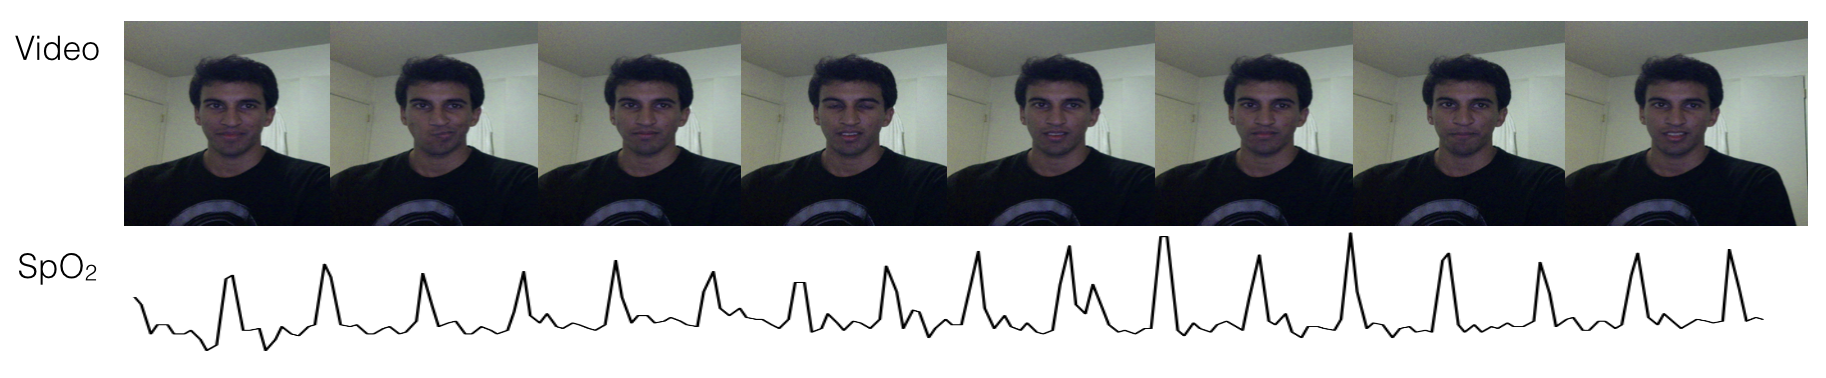
\includegraphics[width=\textwidth]{images/fig3.png}
    \caption{Obtaining ground truth estimates from SpO2 values per image \label{figure:images_and_pulseox}}
  \end{figure}

  Further processing had to be done because the pictures were not taken uniformly in time and so computing a Fourier decomposition of the pixels taken from each image would not be correct.
  An interpolation was needed for images (to create a set of images with uniform time between them) and also for the pulse oximeter data to corroborate with the images.

  In order to accurately train our model, we also needed to bin the pulse oximeter values and be able to recreate the signal from the binned values so that they remained true to life.
  
  


\section{Results and Discussion}
 \subsection*{Initial results}
  At first we took 10 bins over a 6Hz interval of the Fourier transform of each pixel. We outputted a binary vector, with a 1 if the binned value exceeded a threshold and a 0 otherwise. The binning involved with our initial results provided a coarse model and was in fact a very poor representation of the data. In particular, for each pixel the binary vector consisted of [1, 0, 0 ..., 0] which is exactly the same distribution we would expect for noise. Thus our weight matrix contained predominantly zeroes, as we were training to a predominantly zero vector.

  To increase the predictive power of the feature set, we increased the number of bins in the FFT, although limitations in our computational power meant that we were restricted to maximum 24 bins over the 6Hz interval. This applied to both the SpO2 value and the pixel's Fourier transform. We also included the phase terms and the pixel locations as further features (Figure~\ref{figure:preprocessing}).

  \begin{figure}[tb]
    \captionsetup{justification=centering}
    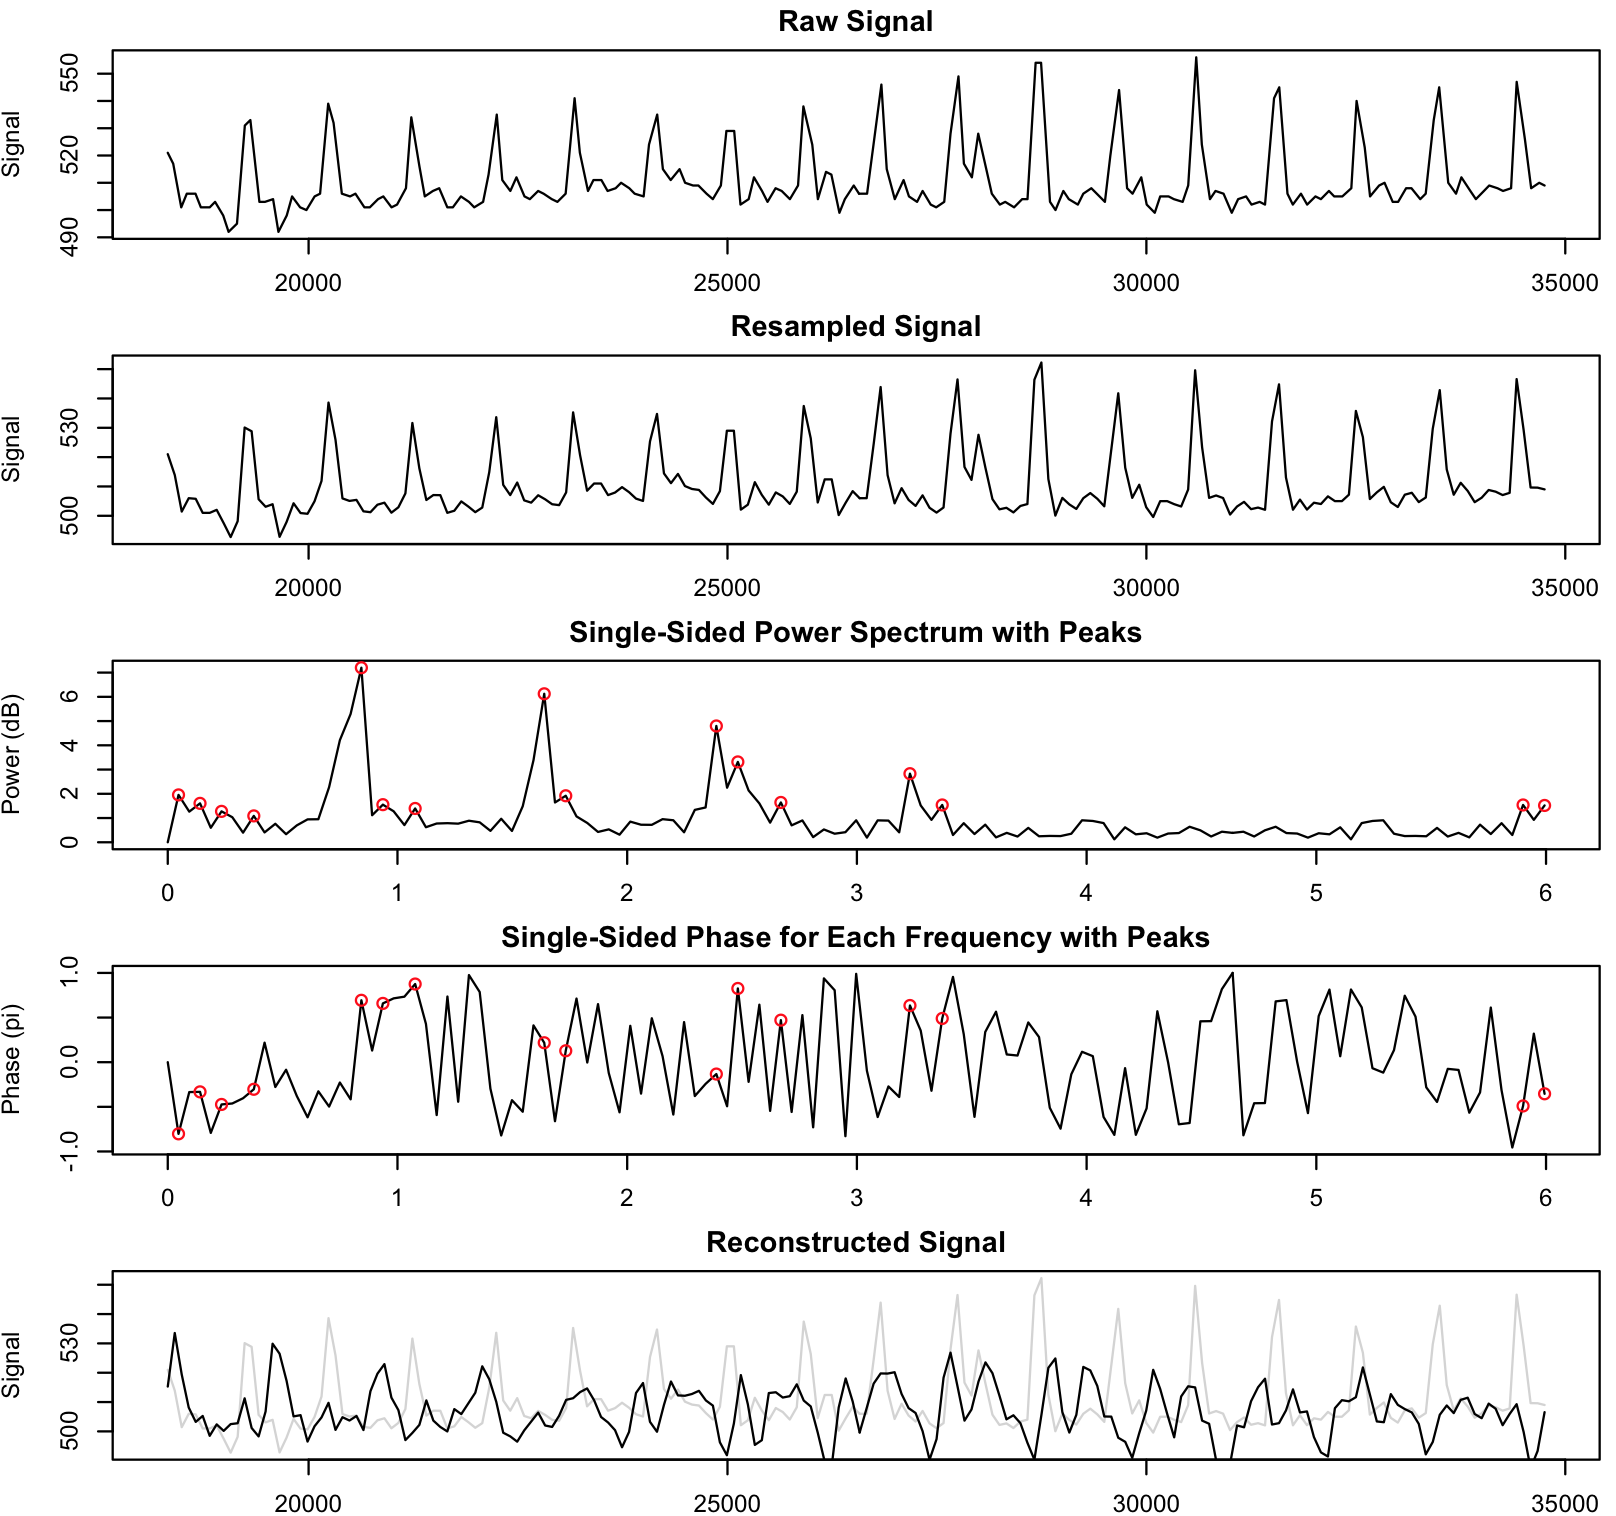
\includegraphics[width=\textwidth]{images/fig1.png}
    \caption{The pre-processing steps \label{figure:preprocessing}}
  \end{figure}
  
 Our feature matrix, \(X\), which contained the features for every training example, gave a matrix $X^TX$ with a very high condition number. This meant the normal equations were unusuable and so stochastic gradient descent was used.
 
 \subsection*{Results}
 Features were extracted from each pixel over time, and included the pixel’s [i,k] location, the FFT of the pixel’s time course binned to 4 buckets per frequencies 0-6Hz [fq1, fq2, …, fq24], and phase [ph1, ph2, …, ph24]. Linear least squares regression models were trained on the combination of features listed in Table 1.\\

\begin{table}[htb]
\begin{center}
\begin{tabular}{|c|c|c|c|c|} 
 \hline
      	\text{Pixel location} & \text{Phase} & 	\text{Frequency} & 	\text{MSE} &  \text{Max cross correlation}  \\ \hline
    	  $\checkmark$ 	&  $\checkmark$ 	&   $\checkmark$ 	& 0.0088 	&  0.0936  \\ \hline
    	   $\checkmark$ 	&  $\checkmark$ 	&   $\times$  	& 0.11 	&  0.0943  \\ \hline
    	   $\checkmark$ 	&  $\times$ 	&   $\checkmark$ 	& 0.0090 	&  0.0936  \\ \hline
    	   $\checkmark$ 	&  $\times$  	&   $\times$ 	& 0.12 	&  0.0943  \\ \hline
    	   $\times$ 	&  $\checkmark$ 	&   $\checkmark$ 	& 0.012 	&  0.0936  \\ \hline
   	   $\times$ 	&  $\checkmark$ 	&   $\times$ 	& 0.75 	&  0.0967  \\ \hline
    	   $\times$ 	&  $\times$  	&   $\checkmark$  	& 0.012  	& 0.0936   \\ \hline
\end{tabular}
\caption{Results of different feature selections with corresponding mean-squared error between predicted and input signal and maximum cross correlation}
\end{center}
\end{table}

These results suggest that each of the features, frequency, phase, and pixel location; play a role in the prediction. Furthermore, the least error was obtained when all three features were used (MSE =0.00884), followed by just frequency and pixel (MSE=0.00903), and pixel location (MSE=0.0117). As expected, for a single video, with numerous pixels serving as training examples, the residuals were low.
  

 \section{Conclusions}
 
 \begin{itemize}

  \item{We built a data collection program that recorded a series of images and SpO2 readings for those images.} 
  \item{Using a binned Fourier Transform, we could efficiently reduce the video data to a finite dimensional feature space and perform regression on it.}
\item{Increasing the variety of features included in the video reduced our mean squared error in the linear regression.}

 \end{itemize}

 \begin{figure}
\captionsetup{justification=raggedright}
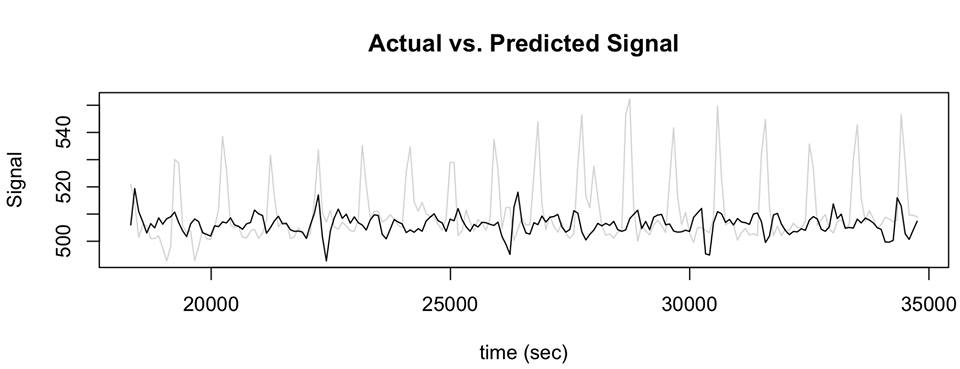
\includegraphics[width=\textwidth]{images/actual_vs_pred_signal.jpg}
\caption{The predicted signal in bold and the actual signal in grey \label{figure:pred}}
\end{figure}

 \section{Further Work}
The main limitation on our method is the encoding process used for reducing the dimension of the training data into features. As can be seen in Figure~\ref{figure:preprocessing} (bottom graph) reconstructing a given signal from its feature set is a lossy process. This in turn increases the noisiness on our predicted signal (Figure~\ref{figure:pred}).


  \bibliographystyle{unsrt} % Plain referencing style
\bibliography{references} %

    %%%%%%%%%%%%%%%%%%%%%%%%%%%%%%%
  \end{document}
  
  